% assignment 3.tex
% Abraham Chan, Cameron Szarapka, Daniel Tan, Sandy Buchanan

\documentclass[journal]{IEEEtran}
\usepackage{float}
\usepackage{graphicx}
\usepackage{amsmath}
\usepackage{enumitem} % For indentation with lists
% correct bad hyphenation
\hyphenation{op-tical net-works semi-conduc-tor}

\date{October 15 2014}
\title{Assignment 3: Virtual Private Network}
\author{Abraham Chan,
	Cameron Szarapka,
	Daniel Tan,
	and Sandy Buchanan}

\begin{document}
\maketitle

% The paper header
\markboth{Department of Electrical and Computer Engineering,
	The University of British Columbia,
	Vancouver, BC, October 15 2014}%
{Shell \MakeLowercase{\textit{et al.}}: Bare Demo of IEEEtran.cls for Journals}

%\begin{abstract}
%The abstract goes here.
%\end{abstract}

\section{Introduction}

\IEEEPARstart{W}{hen} dealing with communications over the Internet, it is important to understand that it is possible for any number of adversaries to intercept, modify, or impersonate communications between any two parties. If privacy is desired for these communications, any messages sent over the Internet must be encrypted. A tool such as a Virtual Private Network (VPN) can be used to allow two parties to communicate while ensuring that the security of the conversation is intact. A VPN ensures that the identity of each party is verified and that the communications between them is encrypted in a secure manner. On top of this, a VPN must also guard against common attacks such as replay attacks or man in the middle attacks and guarantee perfect forward secrecy.

%\section{Instructions for Installation and Execution}
%This needs to be a separate document

\section{Data Transmission and Protection}
Communication between the client and the server in this VPN is accomplished through use of the Windows Socket Application Programming Interface (Winsock API)\cite{sockets}. This API allows for simple establishment of a TCP/IP connection between the client and server over a specified port number. All communications are sent over this unencrypted TCP connection and routed through the Internet. The Winsock API takes care of the fine details behind actually sending and receiving data over the network.

TCP/IP does not offer any encryption by default. Because of this, the VPN must encrypt all data sent between the client and the server. We chose 128-bit AES as the method of encrypting all of the communications over the VPN. AES was chosen because it is accepted as a world wide standard and the accepted form of encryption for many agencies including the US government. The VPN utilizes the OpenSSL implementation of AES, which is open-source. Of all the available modes of operation, the CTR mode of AES is chosen because it is highly parallelizable and therefore better efficiency. The initialization vector (IV) used with the AES-CTR is generated randomly using the OpenSSL "rand" library. The IV used for encryption is then prepended to the ciphertext before being sent over the network.

\section{Mutual Authentication and Key Establishment}
\subsection*{Pre-shared Keys}
The initial communication for this program is accomplished using a key which is agreed upon in advance between the client and the server. This key is essentially the password given to the user of the VPN software to allow them to connect to the server. The password or shared secret value is hashed with a MD5 hash function to obtain a 16-byte key. This key is used only to encrypt the initial communications required to authenticate the user and the server. Also, the shared secret is used as the response to the challenge during authentication to prevent replay attacks.

There are multiple reasons for not using the pre-shared key to encrypt all communications that occur between the client and the server. In the event that the communications are being monitored, using a static pre-shared key over a long period of time can result in an adversary collecting enough data to perform statistical analysis in an attempt to compromise the key. In addition to this, a compromised key, would allow an adversary to decrypt all previously sent messages. This can happen regardless of how the key was compromised. Due to these reasons, using a pre-shared key for all encryption results in a lack of both forward and backward secrecy.

\subsection*{Diffie-Hellman Key Exchange}
An important part of implementing perfect forward secrecy is creating a new key with every session that is established. Using a new encryption key for each session removes the inherent weakness of reusing a pre-shared key. To this end, we implemented a Diffie-Hellman exchange to generate a new shared symmetric key for every new VPN session. The Diffie-Hellman exchange is considered to be secure due to the difficulty of solving the discrete log problem with current computing equipment \cite{dh hardness}.

The Diffie-Hellman exchange was chosen for this project for both its simplicity and its ability to deliver perfect forward and backward secrecy. Every time this exchange is used to create a new session key, there is no relation to any previously generated keys or any future generated keys.

During this exchange, both the server and the client start the process by using a prime number (p) and primitive root modulo (g) generated by the client as well as a secret random number (a, b) to compute a public key as shown in Equation 1, below. This key is then encrypted using a pre-shared key and sent to the other party. Each side then uses this key combined with their secret number to calculate a shared key as shown in Equation 2. This shared key is used for all further encryptions in the session. As a final step to the process, the variables used to generate this shared key are destroyed by the parent process.

\begin{gather}
\mbox{Client computes: }g^{a}\mod{p} \nonumber \\ 
\mbox{Server computes: }g^{b}\mod{p}
\end{gather}

\begin{gather}
\mbox{Client and Server compute: }g^{ab}\mod{p}\\
\nonumber
\end{gather}

In order to prevent this VPN program from being susceptible to man in the middle attacks, the Diffie-Hellman key exchange is encrypted using a pre-shared key and 128-bit AES encryption. This key is only used during the initial exchange, after which the newly established session key is used.

\subsection*{Authentication Handshake}
Authentication for this VPN occurs in three steps. The client contacts the server with a message containing a prime number, the primitive root of that prime, a nonce, and an origin. The server responds to this message with a nonce and a message encrypted with a pre-shared key and containing the client's nonce, an origin message, and a partial session key. The client completes the handshake by responding with a similarly encrypted message containing the server's nonce, an origin message, and the client's partial key. The combination of origin messages, and nonces prevents replay attacks from being used against this program. 

\subsection*{Timed Session Keys}
In an effort to further increase the security of the VPN program, session keys are set to expire after one minute. At this point, a new session key is negotiated and communications may continue. The new session key is established using the previously described Diffie-Hellman exchange. Establishing new session keys on a regular basis ensures that there is never enough data transmitted to allow for statistical analysis of the encryption. This also breaks communications into smaller chunks that will prevent the entire conversation from being revealed if a key is compromised.

\section{Real World Considerations}
If this VPN were a product for sale in the real-world, there are some changes that would be necessary to ensure the desired level of security is achieved. The largest vulnerability that currently exists in this program is in the implementation of the prime number generator. Currently, this function only generates a prime number that is three digits in length. In order to create a cryptographically secure session key, the Diffie-Hellman key generation must be provided with a very large prime number. RFC 3526 provides several ideal candidates towards this end\cite{RFC3526}. Increasing the size of the prime number will allow the Diffie-Hellman exchange to create a secure key which can be used with the existing AES encryption. Due to the fact that this VPN program is only used for secure text communication we feel that increasing the key size of the AES cipher is appropriate. Increasing the key size results in a higher processor load which could prove to be detrimental to high volume data streams. 

\section{Program Details}
\subsection*{Language}
We chose to write the majority of our VPN program in C\# with some parts being written in C. C\# was chosen for its ease of creating a Graphical User Interface (GUI). The implementation of the AES encryption was completed in C due to fact that this language was more familiar to the team and thus easier to use when implementing a complicated function. 
\subsection*{Size}
Our SimpleVPN.exe file is 25 kilobytes in size. It contains 1813 lines of code in 27 files.
\subsection*{Components}
The major components of our VPN are as follows:
\begin{description}
	\item[\bfseries Graphical User Interface] \hfill \\
	The GUI of our VPN is as shown in the figure below.
	\begin{figure}[H]
		\centering
		\caption{SimpleVPN GUI.}
		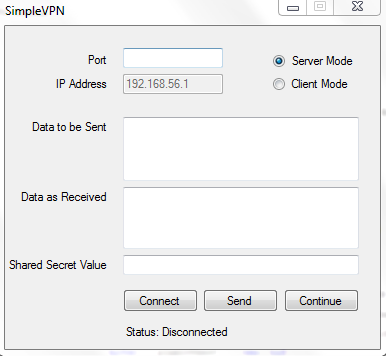
\includegraphics[width=0.5\textwidth]{GUI.png}
	\end{figure}
	Our GUI was built with C\# in Visual Studio Designer.
	As inputs the GUI accepts the user's choice of Client or Server Mode, the Port number, the IP Address of your machine, the data you would like to send to the client/server, and the Shared Secret Value.\\
	As outputs the GUI will display the \emph{Data as Received} from the client/server.% followed by the \emph{Decrypted Received Data}.\\
	For this component, the functionality is as follows. Your choice of Client or Server Mode is determined via radio buttons. The user inputs the Port number into a text box. The IP Address is automatically pulled from system information or can be modified by the user in the text box. The \emph{Data to be Sent} is entered in a text box, sent to our module for encryption along with the \emph{Shared Secret Value}, then sent to the TCP Socket Communication component to be sent to the other client/server.  The TCP Socket Communication component is also the source for the \emph{Data as Received}. % while our encryption module fills our \emph{Decrypted Received Data} field.
	
	\item[\bfseries Encryption/Decryption] \hfill \\
	Our implementation of encryption and decryption incorporates AES and OpenSSL.\\
	As inputs, the module accepts plaintext, the plaintext size, and the session key as converted by OpenSSL. The module outputs ciphertext, the size of cipher text, and the corresponding session key. Of course, the vice versa of this works in order to perform decryption.\\
	The two main functions of this module are the \emph{encrypt} and \emph{decrypt} functions. \emph{encrypt} first initializes the IV with the first 8 bytes as random inputs from OpenSSL's random function and the last 8 bytes. An AES function is then called to set the encryption key. The last block is then padded if it is not a multiple of 16 bytes. Finally the text is prepended with the IV, encrypted using AES CTR mode and the ciphertext is returned. Alternatively, the \emph{decrypt} function begins by extracting the IV from the ciphertext, then calling an AES function to initialize the decryption key. The same AES encryption function is again called to decrypt the ciphertext (by encrypting it with the decrypting key), and the plaintext is returned.
	
	\item[\bfseries Diffie-Hellman Key Exchange] \hfill \\
	The Diffie-Hellman module of the program takes care of creating partial and full session keys. This module takes as inputs a prime number and the corresponding primitive root. The module contains two main functions. The first uses a cryptographic random number generator to create a secret number that is between one and the prime number. As shown in Equation 1 previously, this secret number is used to calculate the partial key which is delivered as the output of this function. The second function takes as input a partial key generated using the same prime / root pair and calculates the full session key using Equation 2 on the previous page.
	The numbers that are generated while doing the calculations in this module are significantly larger than standard 64 bit number types. The BigInteger class in Microsoft's .NET 4.0 framework was used to handle these large numbers. This framework also contained the cryptographic random number generator that was used to create the secret number in this module. 
	
	\item[\bfseries Prime Number Generator] \hfill \\
	The prime generation module of the VPN is used to generate a prime number and primitive root pair for use with the Diffie-Hellman module. This module does not require any inputs. On creation, a cryptographic random number generator is used to select a random prime / root pair from the pre-set table within the module. This table contains all of the three digit prime numbers and their primitive roots. This prime / root pair can be accessed by any function in the program. This module also contains a function that generates a new prime / root pair on demand.
	
	\item[\bfseries Session Key Refresh] \hfill \\
	This module is implemented using a timer class contained within the Microsoft .NET 4.5 framework. The timer was set on creation to refresh the session key once every minute. When the timer elapses, it triggers the authentication module which then generates a new session key. 
	
	\item[\bfseries Authentication and Handshake] \hfill \\
	This module handles the authentication protocol used in this program. When called on the client side, this function creates a nonce and generates a prime / root pair. These are sent to the server along with a byte identifying this side as the client. It then waits for the server's response and replies to that with an encrypted message that includes the received nonce, identifying byte, and partial key. When a handshake is initiated, this module responds to the initial request with a nonce and an encrypted message including the received nonce, identifying byte, and partial key.
	
	\item[\bfseries TCP Bidirectional Socket Communication] \hfill \\
	Our communication module is built on the .NET 4.5 framework. We have created C\# classes for Server and Client Mode inherited from the SocketCommunication class of .NET. These classes give functions taking care of the creating and binding of our sockets given the port from the GUI. After receiving an encrypted message, this module simply sends the package to the other host. To allow for bidirectional communication (allowing the server to send messages to the client) we have made our program multi-threaded. A listener class is run on one thread, listening on the socket while the server is constantly ready to send a message to the client. After sending, the socket on the receiving end will receive encrypted text as its input, and output that to the decryption module to be displayed on our GUI.
	
	\item[\bfseries Hashing] \hfill \\
	The MD5 hash module used in this program is contained within the Microsoft .NET 4.0 framework. This module takes as an input a number and transforms it into a 128 bit hash value. This value is then used as a key for encryption and decryption of message data.
\end{description}

The flow of our VPN program can be shown by the diagram below.
\begin{figure}[H]
	\centering
	\caption{SimpleVPN program flow.}	
	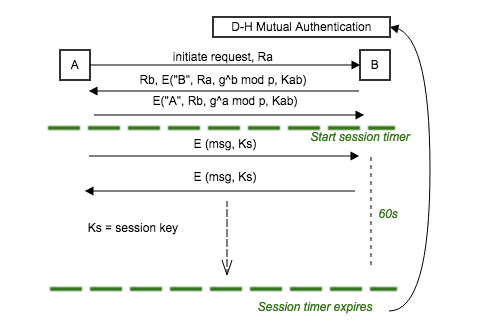
\includegraphics[width=0.5\textwidth]{flow_diagram.png}
\end{figure}

\section{Conclusion}
The VPN created for this assignment contains all of the elements required to ensure that the confidentiality of communications between both users is protected. Perfect forward and backward secrecy is maintained through the use of a Diffie-Hellman key exchange and time expired session keys. Man in the Middle attacks are prevented through encryption of the above key exchange and replay attacks are prevented through the use of a nonce. Even given these precautions, this VPN can not be considered secure. The Diffie-Hellman exchange used in this VPN uses a three digit prime number for computation of the session key. This leaves the VPN using a relatively simple key for encryption of the communications. If this VPN were to be used for secure communications, a much more sophisticated prime number and primitive root computation function would be required.

% references section

\begin{thebibliography}{1}

\bibitem{sockets}
Microsoft, "Windows Sockets 2," Microsoft, [Online]. Available: http://goo.gl/KcgWZ8. [Accessed 10 October 2014].

\bibitem{dh hardness}
A. Joux and K. Nguyen, "Separating Decision Diffie–Hellman from Computational Diffie–Hellman in Cryptographic Groups," Journal of Cryptology, vol. 16, no. 4, pp. 239-247, 2003.

\bibitem{RFC3526}
T. Kivinen and M. Kojo, "More Modular Exponential (MODP) Diffie-Hellman groups for Internet Key Exchange (IKE)", RFC 3526, May 2003. 

\end{thebibliography}

% biography section

\begin{IEEEbiographynophoto}{E-Mails (respectively):}
abrahamchan2@gmail.com,
c.szarapka@gmail.com,
danielkc.tan@yahoo.com,
s.buchanan@alumni.ubc.ca
\end{IEEEbiographynophoto}
%\vfill
%\begin{IEEEbiographynophoto}{Cameron Szarapka}
%c.szarapka@gmail.com
%\end{IEEEbiographynophoto}
%\vfill
%\begin{IEEEbiographynophoto}{Daniel Tan}
%danielkc.tan@yahoo.com
%\end{IEEEbiographynophoto}
%\vfill
%\begin{IEEEbiographynophoto}{Sandy Buchanan}
%s.buchanan@alumni.ubc.ca
%\end{IEEEbiographynophoto}

% that's all folks
\end{document}


